\documentclass[12pt]{article}
\usepackage[utf8]{inputenc}
\usepackage{graphicx}
\usepackage[a4paper,width=150mm,top=25mm,bottom=25mm]{geometry}

\title{Architectural Design Document}
\author{Ctrl Alt Defeat}

\begin{document}
\begin{titlepage}
    \centering



    \vspace{2cm}
    \hrulefill\\
    \vspace{1cm}
    {\Huge\bfseries SRS Documentation v3.0}

    \vspace{1cm}

    {\Large Software Requirements Specification Document for\\Domain Pulse}\\
    \vspace{1cm}
    \hrulefill\\

    \vfill

    {\large Ctrl Alt Defeat}

    \vspace{1cm}

    {\large 2023/07/31}\\
    %    \vspace{1cm}
    %    \vspace{1cm}
    %    
\includegraphics[width=10cm]{../../Images/dpLogo.png}
    %    \vspace{1cm}\\
    %    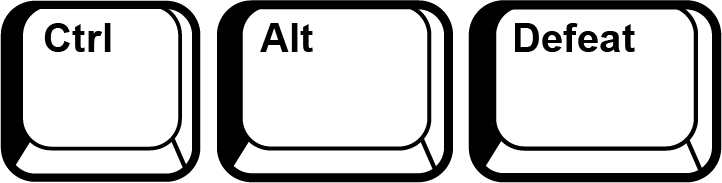
\includegraphics[width=6cm]{../../Images/cadLogo.png}

\end{titlepage}


\tableofcontents
\newpage
\section{Architectural Design Strategy}
\subsection{Approach}
We have opted to follow the approach of: Design based on Quality Requirements
\subsection{Reasons for approach}
\begin{itemize}
    \item This approach allows us to model our system as a solution to an abstract problem (that being the satisfaction of quality requirements). This allows us to  make technology-independent design decisions.
    \item By formulating our design based on quality requirements, we are able to ensure (make a huge step towards ensuring) that the system does indeed meet its quality requirements first and foremost before any code has been written.
    \item By analyzing the system in terms of quality requirements, it becomes clearer which architectural strategies and patterns (discussed below) are most suitable for the system's implementation.
\end{itemize}
\subsection{Reasons to not follow other approaches}
\begin{itemize}
    \item Since our application is dashboard centric, which limits edge case interaction from users, we found it unsuitable to take the approach of designing the system via the generation of test cases. Furthermore, designing test cases would not necessarily help us in identifying approriate architectural stategies and patterns (at least not the the extent that our favoured approach allows)
    \item There are relatively few object-like structures that can be decomposed into suitable hierarchical or relationship structures (at least not to enough of an extent) in our system. Hence we felt that a decomposition approach was not necessarily warranted (at least not over our favoured approach, which we deemed to be the most suitable for our purposes)
\end{itemize}

\newpage
\section{Architectural Quality Requirements}
While almost every possible quality requirement is something that should be aimed for as a general rule, we have identified five quality requirements most important for our system. The quality requirements below are listed in order from the most to "least" prioritised.
\subsection{Usability}
The most essential quality requirement of our system is usability. The target user for our application is not necessarily someone with high proficiency with software systems, sentiment analysis and natural language processing, or IT in general (ex: social media managers, small business and restaurant owners, etc) - consequently, the systems needs to be intuitive and non-overwhelming, both in the user interface as well as in the numerical metrics provided.
\subsection{Security}
As will be explained below, our system will be hosted on a virtual machine on a public IP address - experience and measuring has shown that the network of computers on which the virtual machine lies is subject to up to 17 000 cyber-attacks every 24 hours. Consequently, the security of the system needs to be state of the art in order to prevent would-be attackers from wreaking havoc upon the system. Additionally, in order to ensure the system remains safe and functional, the system needs to be robust and protect against common cyber attacks, as well as protect user data in case of compromise in order to comply with information regulations.
\subsection{Performance}
Performance is an important quality requirement of our system. Our system includes a high degree of data processing and analysing (which can be a time-intensive activity) in addition to the ability to fetch data from external sources (which can also add precious seconds to execution time). Slow performance ruins the user's experience (pertaining to usability) and renders the app more frustrating that useful. 
\subsection{Modifiability}
Ideally, this system will be useful to a fair number of people, who will in turn provide feedback for functionality, sources, and metrics they would like to be able to investigate using the system. Consequently, modifiability of the system is a desirable quality requirement in order to ensure the continuous growth and evolution of the system. 
\subsection{Scalability}
Scalability goes somewhat hand in hand with performance in that the system should not become overly encumbered (resulting in slower performance) when a high number of users are interacting with the system.


\newpage
\section{Architectural Design and Patterns}
\subsection{Diagram}
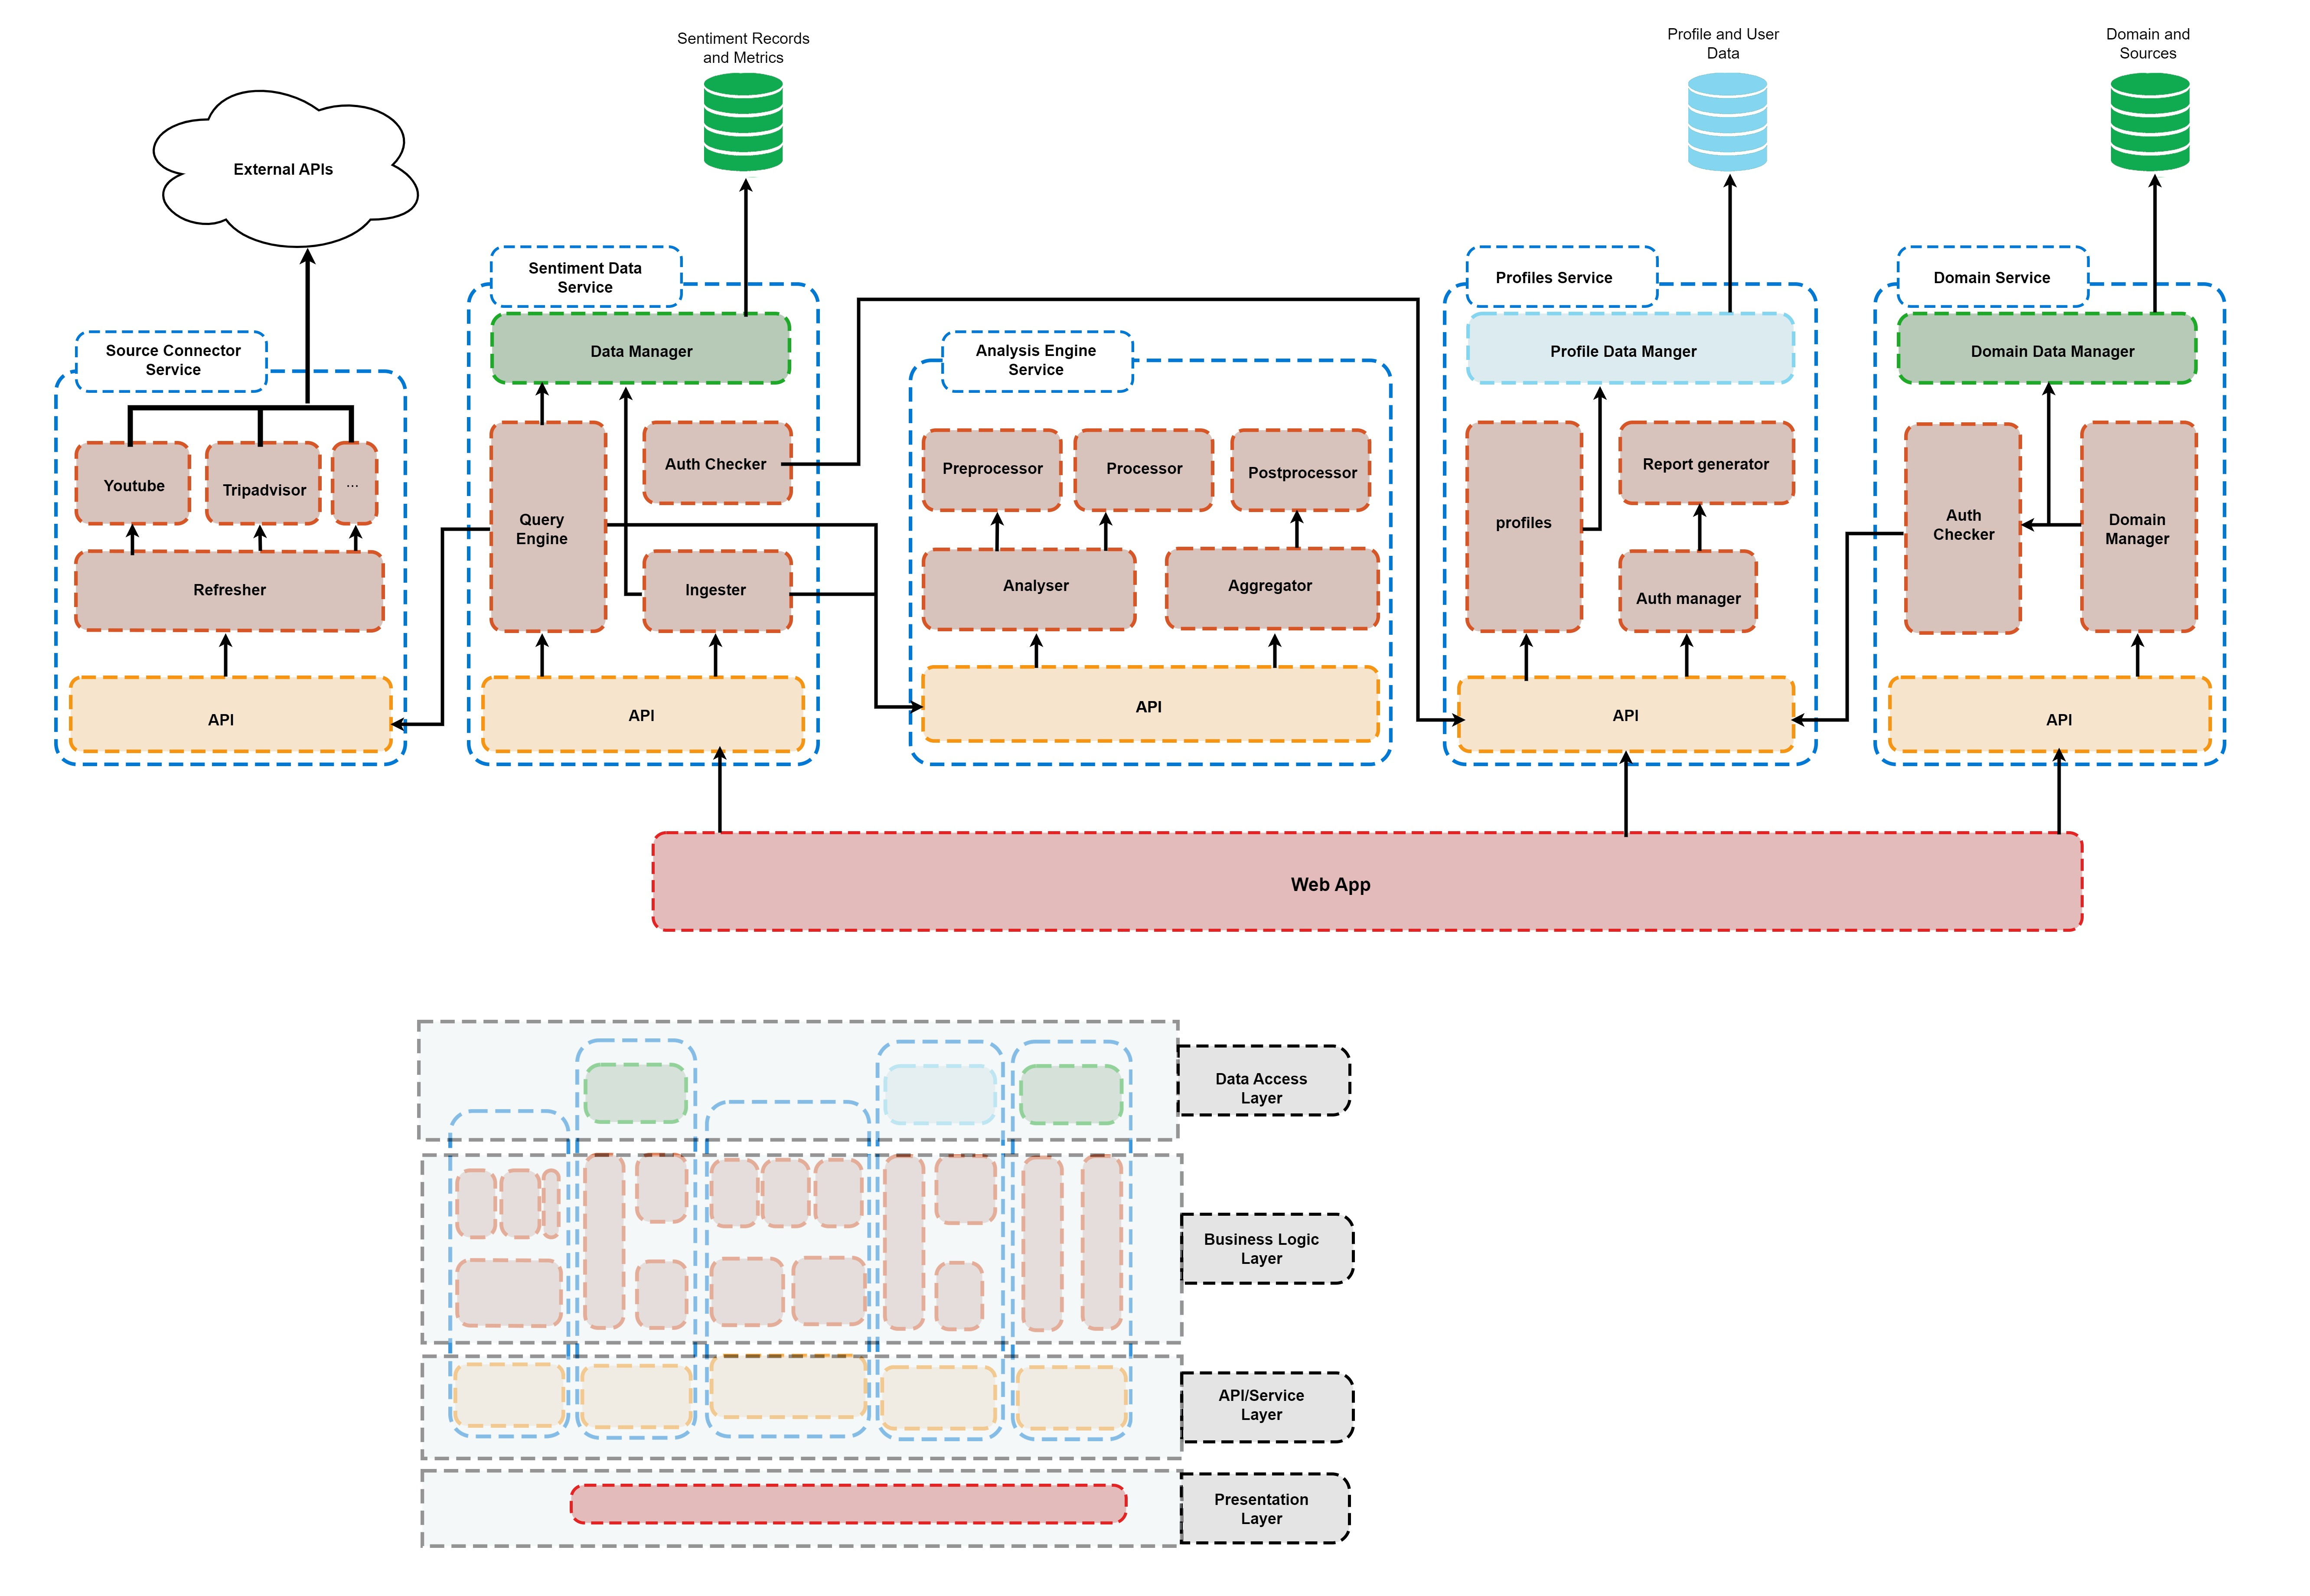
\includegraphics[width=1\textwidth]{Demo4Architecture.jpg}
Please see a description of the employed architectural patterns and tactics below.


\newpage
\section{Architectural Strategies}
We have adopted aspects of several architectural styles, patterns and strategies to help realise our system and its quality requirements. Tactics additionally are grouped by architectural patterns.
\subsection{Service-Oriented Architecture}
\subsubsection{Description}
The overarching software architecture is that of a Service-Oriented Architecture. Our system consists of five different, independently deployable unit, each of which is responsible for providing (a) different services(s).
\subsubsection{Quality Requirements Addressed}
\begin{itemize}
    \item Scalability: The use of a Service-Oriented Architecture promotes scalability of the application by distributing the computational responsibilities across different deployed units (tactic: distributed processing) - thus helping reduce bottleneck.
    \item Performance: The separation of services allows services that require higher computationally expense to be scalled vertically or horizontally (tactic). Furthermore distributed processing of tasks ultimately improves performance.
    \item Modifiability: A SOA takes seperation of concerns (tactic) to an extreme, and allow for individual services to be modified totally independently of one another.
    \item Security: Structuring the application as five independently deployable unit allows for the isolation of components, such that if an attacker compromises a single service, they do not necessarily compromise any of the other services. This isolation helps contain security breaches.
\end{itemize}
\subsection{Multitier/Layered Pattern}
\subsubsection{Description}
A Multitier architecture is achieved by physicaly seperating the modules responsible for presentation, business logic, and data logic. Furthermore, this architecture is Layered in the sense that each layer provides services to the layer below it to use. The layers/tiers are as follows: Presentation layer (frontend UI), Service Layer (public APIs for each service), Business Logic Layer (to handle the application logic), and the Data Access Layer (to handle the database interaction)
\subsubsection{Quality Requirements Addressed}
\begin{itemize}
    \item Modifiability: Once again, seperation of concerns (tactic) is achieved (and is more finely grained) by seperating modules physically by responsibility
    \item General: It is good practice to seperate a system into layers such that updates to one layer in one unit does not affect others. Furthermore this helps realise the Agile methodology which requires that modules are updated and developed rapidly.
\end{itemize}
\subsection{Model-View-Controller Pattern}
\subsubsection{Description}
The use of Angular as a frontend technology (discussed below) inheritedly makes use of the MVC pattern.
\subsubsection{Quality Requirements Addressed}
\begin{itemize}
    \item Usability: By seperating data, visuals, and logic, is it possible to build a highly responsive application with stunning and intuitive visuals.
\end{itemize}
\subsection{Pipe-and-Filter Pattern}
\subsubsection{Description}
The pipe-and-filter architectural pattern is a means to conceptually reason about the sentiment analysis pipeline. The pipeline is as follows: 1. Data is pulled from an external API 2. The data moves through the Query Engine and is formatted and pushed further along the conceptual pipeline 3. The source and/or domain queried is validated as belonging to the user 4. As part of the Analyser, the data is preprocessed using NTK 5. As part of thr Analyser, the data is subject to a number of sentiment analysis models to produce metrics 6. As part of the Aggregator, the data is combined in a meaningful and aggregated manner 7. The next step conceptually is that this fully transformed data is returned to the user on the frontend and presented visually
\subsubsection{Quality Requirements Addressed}
\begin{itemize}
    \item Performance: The use of this conceptual pipeline structure is conducive to parallel processing, an architectural tactic (since this pipeline spans across three different deployable units) improving the time taken for data to be analysed overall on average
    \item Scalabilty: Closing related to performance, the use of a somewhat pipe-and-filter structure allows for pipelining (tactic) in the sense that whille data is in one stage of the pipeline, different data may be simultaneously processed in a different component of the pipeline - improves overall scalability and performance when multiple users are invoking the pipeline simultaneously.
    \item Modifiability: By implementing the sentiment analysis pipeline as a series of filters/components, one can make modifications to one part of the pipeline (ex: preprocessing) without affecting any other stage of the pipeline
\end{itemize}
\subsection{Repository Pattern}
\subsubsection{Description}
As part of the Data layer of the application (see Multitier/Layered Pattern) we have opted to implement the Repository pattern such that we have an intermediary between the databases and the rest of the application. This is doen for all deployable units that include a database (of which there are three).
\subsubsection{Quality Requirements Addressed}
\begin{itemize}
    \item Modifiability: By placing an abstraction between the database and the application logic (tactic), the rest of the system can be totally agnostic of the database technology used, meaning that changes to the database require a minimal amount of code to be changed, namely only the repository/model modules that interact with the database, the rest of the application can remain unchanged.
    \item Performance: Since we can thus guarantee that interaction with the databases takes place in a consistent manner, we can preemptively create optimized database queries (tactic: database optimization) for each predefined database-interaction method defined in the repository/model modules (since the application will always access the databases via these modules). By using optimal queries will the performance of the application improve.
\end{itemize}
\subsection{Important Notice regarding other identified Quality Requirements}
Note that no pattern directly addresses the quality requirement of security. This is because this quality requirement is addressed by the choice of technology (detailed below). Furthermore, the important quality requirement of Usability is only directly addressed via one pattern above - please note however that this is not an oversight. Instead, Usability is so core to our application that it is mainly ingrained into the business logic and technology choices of the system.
\subsubsection{Security}
\begin{itemize}
    \item Authentication is token based (tactic). JWT tokens will be used to authenticate a user across multiple deployed and independent services. These tokens will be verified and managed by a central authentication service (Profiles) - this enables consistent token verification and potentially token blacklisting.
    \item Backend technology choice of Django (discussed below) is designed with security in mind, employing various mechanisms to combat common security vulnerabilities
\end{itemize}
\subsubsection{Usability}
\begin{itemize}
    \item Attention to detail and smooth-ness when designing the UI
    \item Sentiment analysis model outputs are appropriately transformed on the backend such that they are easy to interpret and visualise.
\end{itemize}


\newpage
\section{Architectural Constraints}
\subsection{Client-Defined}
\begin{itemize}
    \item The system needs to consist of at least two seperate deployable units.
    \item The system must be deployed to a virtual machine with a publically available domain name (provided by Southern Cross Solutions). 
    \item The system must make use of at least one NoSQL document-based database
\end{itemize}
\subsection{Hardware and Operating System Constraints}
\begin{itemize}
    \item The system is to be hosted on a single virtual machine (running on a single physical server). At a later date this may be expanded to make use of multiple virtual machines running on different physical machines. This requirement has been relaxed where the use of 3rd party hosting platforms has become necessary.
    \item The system must be suitable for and run on an Ubuntu-style Linux operating system
\end{itemize}

\newpage

\section{Technology Choices}

\subsection{Deployment Techology}
To deploy our application we use docker and its accomppannying set of technologies.
\subsubsection{Docker Engine}
    For each of our backend services we define a Dockerfile which defines the python environment and dependencies needed for the service to run.
    \newline IMAGE OF DOCKER IMAGES
\subsubsection{Docker Compose}
    To manage the deployment of our services and how how they communicate we use docker compose.
    \newline Docker compose allows us to define a set of services and how they communicate with each other in a docker-compose.yml file.
    \newline We use the docker compose file to inject the environment variables needed for our services to fucntion at run time.
\subsection{Github workflows}
    We use github workflows to automate the deployment of our application to the servers we use.
    \newline For each of the services there is a workflows defined that does the following
    \begin{itemize}
        \item Inject the repository secrets needed to connect to our servers into the action runner
        \item use a cache of the dependencies needed to run tests to decrease ci/cd times
        \item run tests on the service
        \item build the docker image for the service and push to docker hub
    \end{itemize}
    It is inefficent to always build the docker image and push that becuase the docker image would only change when the code in the specific service changes.
    \newline So what we do to speed up the ci/cd process is use git diff to see whether code in the specific folder of the service has changed, only then does the image get built and pushed to docker hub.
    \newline IMAGE OF GITHUB WOKFLOW PROCESS
    \newline IMAGE OF DEPLOYMENT DIAGRAM (showing all the services, where they live and what they run on)

\subsection{Frontend Technology}
Our frontend consists of the use of Angular which is an open source web application development framework that was developed by google. Angular is used to build dynamic and responsive applications.
\subsubsection{Angular}
The reasons below are some of the key points as to why Angular is best suited for our application
\begin{itemize}
    \item Angular is a complete framework which means that it doesnt have to rely on any other frameworks to complete any functionality front end wise , this is good because we already have multiple deployable units and having a singular front end framework would be a great way to declutter the project and not have a steep learning curve with multiple frontend frameworks.
    \item Angular promotes a Component based architecture which is great in terms of our project because as mentioned above we have multiple deployable units and as Angular promotes component-based architectures this will be good as we will require modularity, code reusability and separation of concerns.
    \item Angular has a large component for testing, including unit tests, integration tests and end to end tests, Angular makes use of Jasmine and Karma for writing and running tests which allows for higher quality and reliablity of applications developed with Angular
\end{itemize}
In contrast there are always drawbacks to all technology and below are some of the shortcomings
\begin{itemize}
    \item Angular has a larger file size when compared to other frameworks, the initial bundle of Angular is much larger in size and can result in lomger loading times and slower network connections.
    \item Angular has a steep learning curve in general when compared to other frameworks such as React which has core components that are easy to grasp.
    \item Angular is complex, it has many features and its complexity can lead to its downfall in terms of development time and overly detailed or long code.
\end{itemize}
The argument about how Angular is more fit for our project is presented below:
\begin{itemize}
    \item Angular is a good fit for good fit for our architecture as it has built in common practice ways of interacting with multiple backends, angular also provides a good framework for building abstractions on top of a service oriented architecture. 
    \item Angulars component based architecture and dependancy injection system pair well with the principles of service orientated architecture,such that in a service orientated architecture applications are structured as a collection of loosly coupled services that communicate with each other through interfaces
    \item Angulars approach to the information above is that its components can be designed to encapsulate specific functionalities or services within the application.
    \item The steep learning curve of Angular is offset by the fact that all Ctrl Alt Defeat developers have experience with Angular already from previous projects.
\end{itemize}
With the above describes why we have opted for Angular.
\subsubsection{React}
React is library developed by Facebook for building user interfaces.
Advantages of react:
\begin{itemize}
    \item React uses a virtual DOM which efficiently updates and renders only the components that have changed.
    \item One way data flow which promotes data consistency
\end{itemize}
Disadvantages of react:
\begin{itemize}
    \item Significant boilerplate code
    \item Rapidly evolving ecosystem
\end{itemize}
We decided against using React because of the amount of unused boilerplate code in addition to lack of developer experience with the technology.

\subsubsection{Svelte}
Svelte is a JavaScript framework that takes a different approach to building user interfaces compared to traditional frameworks.
\begin{itemize}
    \item Highly optimised code leads to high performance
    \item Framework-less does not rely on a runtime library
\end{itemize}
Disadvantages to Svelte:
\begin{itemize}
    \item Limited ecosystem and small community
    \item Steep learning curve for advanced features
\end{itemize}
We decided against Svelte due to the the limited integration tools it has as well as steep learning curve.

\subsection{Backend Technology}

Our backend consists of five different deployable units, each developed using Django to perform the business logic, data logic, and API functionality. The reasoning behind this technology choice is explained below.
\subsubsection{Django}
The following reasons are the main driving force this design decision:
\begin{itemize}
    \item Django is a high-level Python web framework that follows the Model-View-Controller (MVC) architectural pattern. It provides a robust and efficient toolkit for building web applications.
\end{itemize}
\begin{itemize}
    \item Django is, by design, highly secure 'out of the box' and provides comprehensive protection for all the most common security threats (SQL injection, CSRF, clickjacking, etc). This is of particularly high value to us since (as pointed out in the architectural constraints) the system will be hosted on a virtual machine with a public IP that is subject to frequent cyber-attacks. In order to minimize risk wrought on by inexperience or oversight, a highly secure framework such as Django is a very suitable choice for our purposes.
    \item Django is an entirely Python development environment. Since our system includes a significant portion of data manipulation (across all services), Python will improve the ease with which we are able to develop the system. Furthermore, Python has a number of fantastic libraries for Natural Language Processing and Machine Learning (ex: NLTK, PyTorch, etc), this language is a great choice to handle the application's sentiment analysis component. Additionally, all group members have high proficiency with Python, allowing us to lean into our strengths as programmers.
    \item Django is designed for rapid and smooth development, this is suitable and desirable since we are adopting the Agile Software Process. That is, by developing our system using Django, we are able to rapidly prototype and build on different aspects of our system - allowing for maximum flexibility, while speeding up iteration-by-iteration improvement (highly desirable and necessary trait to successfully adopt the Agile process)
    \item Compared to other frameworks like ASP.NET and Express.js django has an elegant codebase which allows for clean and maintainable code and has a very versiaile ORM (object relational mapping) is great for our 3 databases as we have to optimise everything we can in terms of database querying , storing etc
\end{itemize}
However, no technology choice is ever perfect and there are some trade-offs which need to be minimized.
\begin{itemize}
    \item Django accomplishes the advantages pointed out by points 1 and 3 above by being a 'batteries included' framework. Unfortunately this means that Django is more heavyweight than other Python frameworks such as Flask. A more lightweight framework may be more desirable since we are adopting a service-oriented architecture (ie: not every service will have use of all of Django's built-in features). We do however believe that the advantages described above outweigh this point, since each service in the architecture will leverage at least a few of Django's native features to great effect.
    \item Django is somewhat opinionated about the structure of the application which once again is not particularly desirable for a service-oriented architecture - however, this point is easily negated as it is entirely possible (and fairly easy) to add (through the use of user-defined Python modules) and remove components to accomplish our architectural structure.
\end{itemize}
The argument on why we have chosen django is presented below:
\begin{itemize}
    \item One of our constraints is that we have to use a NoSQL database and Django integrates well with this databse as djago provides a Object-Relational mapping which allows developers to interact with the database using python objects. Djangos modularity and component based architecture make it well suited for building services within an SOA , Django component can be reused and comunicate with eachother through interfaces.Django includes built in authentication and authorization which can be highly leveraged in an SOA architecture , Django can handle high traffic and scale well when deployed as it has functionality for load balancing,caching and database optimization.
\end{itemize}

\subsubsection{Flask}
Flask is a lightweight and flexible web framework for Python. It provides a simple and minimalist approach to building web applications.
Advantages of flask:
\begin{itemize}
    \item Easy to learn
    \item It has a small core framework and provides only essential features
\end{itemize}
Disadvantages of Flask:
\begin{itemize}
    \item Doesn't have a lot of functionality and is very "light-weight"
\end{itemize}
We decided against using flask because it lacks built-in functionality that will improve our development speed.
\subsubsection{Express.js}
Express.js is a minimal and flexible Node.js web application framework that provides a robust set of features for web and mobile applications.
Advantages of express.js:
\begin{itemize}
    \item Minimalistic and lightweight
    \item Has middleware support
\end{itemize}
Disadvantages of Express.js:
\begin{itemize}
    \item Minimalistic approach is not ideal for complex projects
\end{itemize}
We opted against express.js since it is minimalistic and we require more built-in functionality to be able to rapidly develop our application in accordance with Agile methodologies.
\subsection{Database Technology}
\begin{itemize}
    \item A NoSQL (Not Only SQL) database is a type of database that provides a non-relational, schema-less approach to data storage and retrieval. Unlike traditional relational databases, NoSQL databases are designed to handle large volumes of unstructured or semi-structured data and offer flexible data models.
    \item PostgreSQL is a powerful and highly reliable relational database that adheres to ACID (Atomicity, Consistency, Isolation, Durability) principles. It organizes data into tables with predefined schemas, where relationships can be established between tables using foreign keys.
\end{itemize}
Our system comprises three seperate databases, each running on different deployable units and each serve a different purpose. The description and reasoning of each is below.
\subsubsection{Sentiment Records Database}
This is a NoSQL document-based MongoDB database that runs on the Data Warehouse deployable unit. It is the main and largest database on the application, and contains all the sentiment records/data that have been analyzed, as well as the sentiment metrics that have been computed for each record.
\begin{itemize}
    \item A NoSQL database lends itself to this data because of unpredictable size and variety of the sentiment records that are retrieved online.
    \item Furthermore, the metrics that are computed for each record are closely tied to the record itself (since the record will never be accessed outside the context of checking the sentiment metrics). By leveraging the document structure allowed by MongoDB, it is possible to store both the data and the metrics as a single document/unit.
    \item Potentially most importantly, a NoSQL database (especially the document-based MongoDB) allows for flexibility and modifiability of the metrics computed on a particular sentiment record. For example, in the future it may be desirable to include an objectivity-subjectivity score on new articles that have been analysed. The flexibility of MongoDB would make this modification extremely simple, as no change needs to be applied to the database schema, or to any of the other existing documents in the database.
\end{itemize}
\subsubsection{Domains and Sources Database}
This is a NoSQL document-based MongoDB database that runs on the Domains deployable unit. It is responsible for storing the information and structure of a domain, as well as the sources specified within it (including the information and parameters for those sources)
\begin{itemize}
    \item Since domains effectively act as 'folders' for sources, MongoDB is once again a suitable choice of technology, as it allows us to store sources as nested objects within a domain (which is the document). This helps accomplish 1. domains physically group their associated sources (and easily catering for a variable number of sources), as opposed to a SQL approach, which would alomost certainly require the use of complex joins, and 2. accomplish some form of query/database optimization in that since domains will ALWAYS be accessed in order to retrieve ALL their contained sources, we avoid consistently having to use joins like we would in a SQL databasee, instead by retrieving a single document (domain) we have all the information we required.
    \item Furthermore since the parameters for different sources vary both in number and in type/name, by leverage a MongoDB database we do not need to create some static schema that needs to cater for all possible parameters. Instead we can simple create an object that contains key value pairs of the parameter name and its value.
\end{itemize}
\subsubsection{Profiles, Users, and Authentication}
This is a SQL Postgre database that runs on the Profiles deployable unit. It is resposible for storing a user's profile information and preferences, linking it to their domains in the above database, and managing user and authentication data.
\begin{itemize}
    \item The data to be stored by this database is highly structured and well-defined, and consequently a SQL database is highly suitable for this purpose.
    \item Additionally, Django (backend technology) provides seemless and secure integration with Postgre 'right out of the box' and hence we are able to leverage this predefined interaction in our development. (It is worth noting that this seemless integration is designed with security in mind, providing appropriate and comprehensive protection for database attacks such as SQL Injection)
\end{itemize}
The reason we have chosen these 2 types of databases is because of the following:
\begin{itemize}
    \item PostgreSQL database is a great choice for service-oriented architecture because of its flexibility and extensibility , postgres is highly flexible and extensible DBMS , supports a wide range od data types and the flexibility allows for models and storage of diverse data formats making it great for all different needs of an SOA. The improved flexibility enables easier modifiability.
    \item A PostgreSQL has good scalability and performance and postgre is known for its capabilities in these areas, it can handle high transaction loads and large datasets with proper configuration and optimization , because our project has 3 databases postgre will be great when needing to minimize time spent interacting with the databases as it also has functionality for query optimization and parallel execution.
\end{itemize}
\subsubsection{File Uploading and Storage}
This is a Azure cloud based file storage solution. It is responsible for storing image uploads from users and providing the URLs for the application to access the images.
\begin{itemize}
    \item Since the files to be stored are not particularly large, and since the files are not particularly important (ie: they are not critical to the functioning of the application), a cloud storage solution is a suitable choice.
\end{itemize}
The reason we have chosen this types of cloud storage:
\begin{itemize}
    \item Azure's cloud storage is simple and quick to set up, and allows for easy integration with our frontend techinology (Angular/Typescript).
\end{itemize}
\subsection{Alternatives for database technology}
\begin{itemize}
    \item Alternative for postgreSQL is MySQL
    \item Alternative for MongoDB is CouchDB
\end{itemize}
Advantages for MySQL:
\begin{itemize}
    \item Wide adoption and community support
    \item good performance and scalibility
\end{itemize}
Disadvantages for MySQL:
\begin{itemize}
    \item Not as flexible as postgreSQL
    \item Not as secure as postgreSQL
\end{itemize}
Advantages for CouchDB:
\begin{itemize}
    \item Multiversion concurrency control
    \item Great fault tolerance and availability
\end{itemize}
Disadvantages for CouchDB:
\begin{itemize}
    \item Poor performance on large data sets
    \item Does not have good advanced querying functionality
\end{itemize}
with the above reasons we decided to use postgreSQL and MongoDB
\end{document}